\section{Proposed Methodology}
\subsection{Problem Formulation}
Let $X_t \in \mathbb{R}^{5 \times 28}$ denote a 5-step sequence tensor of 28 features representing telemetry history from time step $t-4$ to $t$ (a 10-hour lookback window). The predictive objective is to learn a parameterized function $f_\theta: X_t \to \hat{y}_{t+1}$ mapping sequence tensor $X_t$ to a multi-class risk probability distribution over target classes $\mathcal{Y} = \{\text{Low}, \text{Medium}, \text{High}\}$ at forecast horizon $T+2\text{h}$.

\subsection{Informer Architecture Formulation}
The Informer sequence model \cite{zhou2021informer} addresses the quadratic computational bottleneck of canonical self-attention mechanisms through three architectural innovations:
\begin{enumerate}
    \item \textbf{ProbSparse Self-Attention:} Computes attention scores selectively on dominant Query vectors using a KL-divergence measurement, reducing time and memory complexity from $O(L^2)$ to $O(L \log L)$.
    \item \textbf{Self-Attention Distilling:} Uses 1D max-pooling layers with stride 2 between attention blocks to halve feature sequence lengths iteratively, extracting dominant temporal features and reducing memory footprint.
    \item \textbf{Generative Style Decoder:} Receives long sequence inputs and predicts target horizon steps in a single forward pass, preventing cumulative error propagation.
\end{enumerate}

In our implementation, input tensor $X_t \in \mathbb{R}^{B \times 5 \times 28}$ is projected into embedding space ($d_{\text{model}} = 64$) via a linear layer. The projected tensor passes through 4-head ProbSparse multi-head self-attention layers with Dropout ($0.2$). A dense classification projection layer maps flattened sequence representations ($64 \times 5 = 320 \to 128 \to 3$) to produce Softmax risk logits.

Fig. \ref{fig:sys_arch} illustrates the end-to-end system architecture of SmartGrid Sentinel, spanning data ingestion, feature engineering, sequence modeling, rule-based explanation, and deployment alert endpoints.

\begin{figure*}[htbp]
\centering
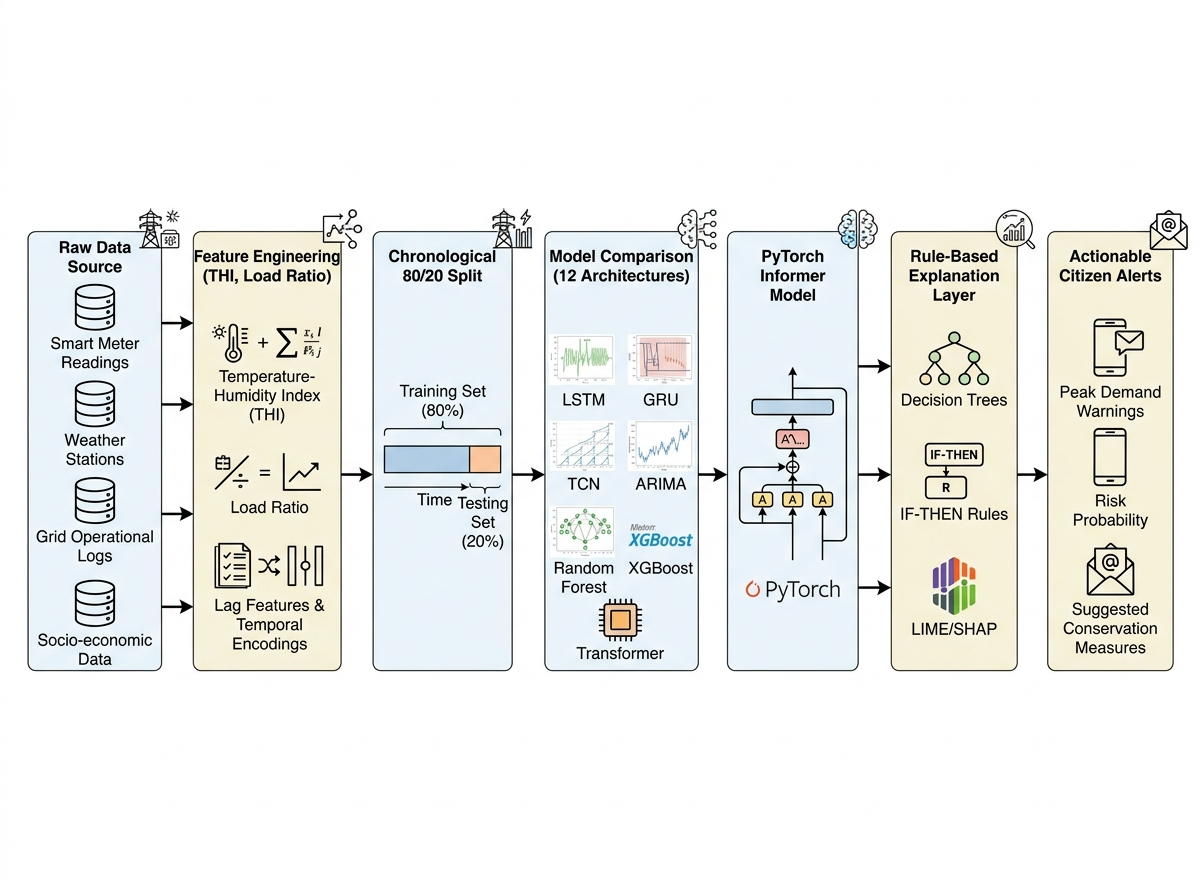
\includegraphics[width=0.92\textwidth]{figures/fig1_system_architecture.jpg}
\caption{End-to-End System Architecture of SmartGrid Sentinel.}
\label{fig:sys_arch}
\end{figure*}
